%%%%%%%%%%%%%%%%%%%%%%%%%%%%%%%%%%%%%%%%%%%%%%%%%%%%%%%%%%%%%%%%%%%%%%%%%%%%%%%%%%%%%%%%%%%%%%%%%%%%%%%%%%
% SCStack
%%%%%%%%%%%%%%%%%%%%%%%%%%%%%%%%%%%%%%%%%%%%%%%%%%%%%%%%%%%%%%%%%%%%%%%%%%%%%%%%%%%%%%%%%%%%%%%%%%%%%%%%%%

\chapter{SCStack}
\label{chap:scstack}

\par SCStack es el conjunto de herramientas que componen la Forja de desarrollo. La palabra \emph{stack} en Inglés significa \emph{pila}, con respecto a la forja se trata del conjunto de herramientas apiladas y conectadas que dan forma a la Forja.

\begin{figure}[H]
    \centering
    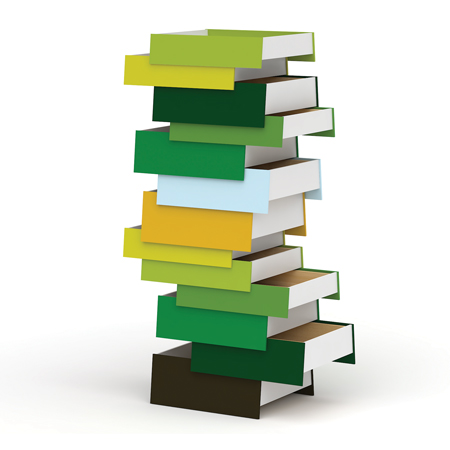
\includegraphics[width=0.7\textwidth]{stackstorage}
    \caption{Ejemplo de pila a partir de cajones}
    \label{fig:stackstorage}
\end{figure}

\section{Arquitectura}
\label{sec:arquitectura}

\par La arquitectura del Sistema de Gestión de la Forja se ve reflejada en el siguiente esquema:

% TODO Imagen UI -> REST Server -> API

\par El proyecto consta de tres componentes conectados entre sí para la comunicación del usuario con las herramientas para la gestión de los proyectos: La Consola de Administración, el servidor de servicios web REST y el API.

%%%%%%%%%%%%%%%%%%%%%%%%%%%%%%%%%%%%%%%%%%%%%%%%%%%%%%%%%%%%%%%%%%%%%%%%%%%%%%%%%%%%%%%%%%%%%%%%%%%%%%%%%%
% Consola de Administración
%%%%%%%%%%%%%%%%%%%%%%%%%%%%%%%%%%%%%%%%%%%%%%%%%%%%%%%%%%%%%%%%%%%%%%%%%%%%%%%%%%%%%%%%%%%%%%%%%%%%%%%%%%

\subsection{Consola de Administración}
\label{sub:consola-admin}

\par \textbf{Consola de Administración}: Se trata de la capa de la vista encargada de interactuar con el usuario. A través de la interfaz que se ejecuta sobre un navegador web, el usuario administrador gestiona los usuarios y los proyectos de la Forja: crear, editar, modificar, eliminar y buscar), el típico sistema CRUD-F\footnote{\url{http://en.wikipedia.org/wiki/Create,\_read,\_update\_and\_delete}} (\emph{CRUD: Create, Read, Update and Delete also Find}). Está diseñada con el framework Javascript \emph{jQuery} por lo que no requiere ninguna librería externa para su uso, únicamente el navegador del cliente. Las operaciones que se realizan en la capa UI se trasladan al servidor REST a través de peticiones \emph{http} asíncronas mediante las interfaces REST definidas.

% subsection consola-admin (end)

%%%%%%%%%%%%%%%%%%%%%%%%%%%%%%%%%%%%%%%%%%%%%%%%%%%%%%%%%%%%%%%%%%%%%%%%%%%%%%%%%%%%%%%%%%%%%%%%%%%%%%%%%%
% Servicio web REST
%%%%%%%%%%%%%%%%%%%%%%%%%%%%%%%%%%%%%%%%%%%%%%%%%%%%%%%%%%%%%%%%%%%%%%%%%%%%%%%%%%%%%%%%%%%%%%%%%%%%%%%%%%

\subsection{Servicio web REST}
\label{sub:rest-ws}

\par \emph{REST}: Representational State Transfer se trata de una arquitectura acuñada por \emph{Roy Fielding}\footnote{\url{http://roy.gbiv.com/}}, uno de los autores de la especificación del protocolo \emph{HTTP}. Esta arquitectura de comunicación se basa en cuatro principios:

\begin{itemize}
	\item Un protocolo cliente/servidor \emph{sin estado}: cada mensaje HTTP contiene toda la información necesaria para comprender la petición. Como resultado, ni el cliente ni el servidor necesitan recordar ningún estado de las comunicaciones entre mensajes. Sin embargo, en la práctica, muchas aplicaciones basadas en HTTP utilizan cookies y otros mecanismos para mantener el estado de la sesión.

	\item Un \emph{conjunto de operaciones} bien definidas que se aplican a todos los recursos de información: HTTP en sí define un conjunto pequeño de operaciones, las más importantes son \textbf{POST}, \textbf{GET}, \textbf{PUT} y \textbf{DELETE}.

	\item Una sintaxis \emph{universal} para identificar los recursos. En un sistema REST, cada recurso es direccionable únicamente a través de su URI.

	\item El uso de \emph{hipermedios}: tanto para la información de la aplicación como para las transiciones de estado de la aplicación. Como resultado de esto, es posible navegar de un recurso REST a muchos otros, simplemente siguiendo enlaces sin requerir el uso de registros u otra infraestructura adicional.
\end{itemize}

\par El uso de los servicios REST para la comunicación mediante el protocolo http con la Consola de Administración agiliza la adaptación de la funcionalidades al cliente, el tráfico y las posibles adaptaciones de nuevos clientes para el acceso a través de cualquier plataforma.

\begin{figure}[H]
    \centering
    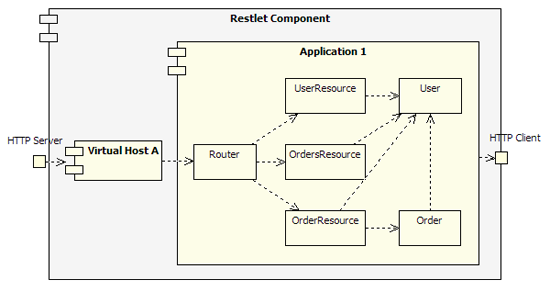
\includegraphics[width=1\textwidth]{restlet}
    \caption{Diseño de un API RESTful}
    \label{fig:restful-api}
\end{figure}

\par \textbf{Servicio web REST}: Es el componente encargado de gestionar las peticiones http a los servicios REST de la Consola de Administración y el API de SidelabCode. Define e implementa la lógica a seguir para la construcción de un proyecto a través de la UI mediante las llamadas ordenadas al API de cada una de las herramientas involucradas en el servicio como componentes de la forja.

\par Los servicios REST ofrecen tres interfaces distintas accesibles a través de http: XML, JSON y HTML para la comunicación la API. Además, hay que desatacar que el servicio web es servido a través del framework \emph{Restlet} a través de Internet de forma continua y remota a cualquier usuario o proceso cliente.

\par Se encarga de la seguridad y validación para las operaciones permitidas o denegadas del usuario de la UI, proporcionando, según su rol, determinados servicios a través de la Consola de Administración, buscar proyectos, crear usuarios, editar proyectos, crear proyectos, etc.

% subsection rest-ws (end)

%%%%%%%%%%%%%%%%%%%%%%%%%%%%%%%%%%%%%%%%%%%%%%%%%%%%%%%%%%%%%%%%%%%%%%%%%%%%%%%%%%%%%%%%%%%%%%%%%%%%%%%%%%
% API
%%%%%%%%%%%%%%%%%%%%%%%%%%%%%%%%%%%%%%%%%%%%%%%%%%%%%%%%%%%%%%%%%%%%%%%%%%%%%%%%%%%%%%%%%%%%%%%%%%%%%%%%%%

\subsection{API}
\label{sub:api}

\par \textbf{API}: La API es el núcleo funcional de SCStack, coordina y realiza las tareas para cada componente de la forja con respecto a los usuarios y proyectos involucrados. Traslada las órdenes ejecutadas en la capa UI a las distintas herramientas para configurar su funcionamiento. Está conectada a todos los servicios que ofrece pivotando a través del directorio LDAP: Control de Versiones, Directorios, Integración Continua, ITS, Revisiones, Gestión de Dependencias, Seguridad y Autenticación que analizaremos extensamente más adelante componente a componente.

% subsection api (end)

% section arquitectura (end)

%%%%%%%%%%%%%%%%%%%%%%%%%%%%%%%%%%%%%%%%%%%%%%%%%%%%%%%%%%%%%%%%%%%%%%%%%%%%%%%%%%%%%%%%%%%%%%%%%%%%%%%%%%
% Aprovisionamiento (Puppet)
%%%%%%%%%%%%%%%%%%%%%%%%%%%%%%%%%%%%%%%%%%%%%%%%%%%%%%%%%%%%%%%%%%%%%%%%%%%%%%%%%%%%%%%%%%%%%%%%%%%%%%%%%%

\section{Aprovisionamiento (Puppet)}
\label{sec:puppet}

\par \emph{Aprovisionamiento}: 'Accción o efecto de aprovisionar', \emph{aprovisionar}: abastecer\footnote{Definición del diccionario de la RAE - \url{http://buscon.rae.es/drae/?type=3&val=aprovisionar&val_aux=&origen=REDRAE}}. Aplicado a la Ingeniería del Software el Aprovisionamiento nos provee de los componentes necesarias para construir una solución.

\par El aprovisionamiento trata de la automatización de tareas para construir el entorno deseado, en este caso la instalación de SidelabCode Stack. La evolución en el modelo de instalación para facilitar la ejecución de módulos, configuración y comunicación entre los distintos componentes.

\par La herramienta empleada para el aprovisionamiento es \textbf{Puppet} de la compañía \emph{PuppetLabs}\footnote{\url{https://puppetlabs.com/}}.

\begin{figure}[H]
    \centering
    
\includegraphics[width=0.7\textwidth]{puppet-labs-logo}
    \caption{Puppet Labs Logo}
    \label{fig:puppet-labs}
\end{figure}

\par \emph{Puppet}: es una herramienta \emph{Software Libre}\footnote{\url{https://puppetlabs.com/puppet/puppet-open-source/}} de aprovisionamiento desarrollada en \emph{Ruby}\footnote{\url{https://github.com/puppetlabs/puppet}}. Gestiona la infraestructura a través de su ciclo de vida, desde el aprovisionamiento y la configuración de parches automatizando la ejecución de órdenes para la instalación y configuración del entorno.

\begin{itemize}
	\item Automatizar tareas repetitivas.
	\item Desplegar rápidamente aplicaciones críticas.
	\item Gestionar proactivamente el cambio.
	\item Escalar de 10 servidores para 1000.
	\item Instalaciones locales o en la nube.
\end{itemize}

\par \emph{Puppet} utiliza un enfoque declarativo, basado en el modelo de automatización:
\begin{itemize}
	\item \emph{Definir} el estado deseado de la configuración de la infraestructura mediante lenguaje de configuración declarativa de Puppet.
	\item \emph{Simular} los cambios de configuración antes de la ejecución.
	\item \emph{Corroborar} el estado final mediante despliegues automáticos comprobando las posibles desviaciones en la configuración.
	\item \emph{Informe} sobre las diferencias entre los estados reales y deseados y cualquier cambio que haya hecho cumplir el estado deseado.
\end{itemize}

\begin{figure}[H]
    \centering
    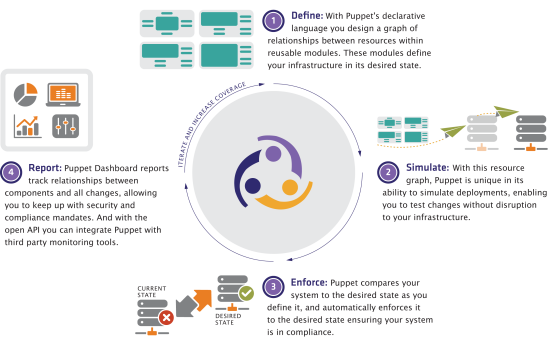
\includegraphics[width=0.7\textwidth]{howpuppetworks}
    \caption{Ciclo de vida de los módulos Puppet}
    \label{fig:howpuppetworks}
\end{figure}

\par El diseño del aprovisionamiento a través de Puppet se basa en módulos. Cada uno de estos módulos se encarga de gestionar la instalación y configuración del componente definido.

\par Que aporta Puppet ? Proporciona un control sobre la instalación de cada herramienta y la configuración asociada por defecto que se define. De esta forma el proceso se instalación se automatiza permitiendo la replicación del mismo, completo o por módulos en diferentes entornos, locales o virtuales. La instalación a partir de módulos ha de definir una cadena de dependencias entre cada uno de ellos de manera que se vayan habilitando funcionalidades e interacciones (Apéndice ~\ref{app:apendice-puppet}).

\par En SidelabCode Stack Puppet es el encargado de gestionar la \emph{instalación y configuración} de cada uno de los componentes mediante módulos Puppet independientes para completar el proceso de instalación (Apéndice ~\ref{app:instalacion-sidelab}) entre 5 y 10 minutos.

%%%%%%%%%%%%%%%%%%%%%%%%%%%%%%%%%%%%%%%%%%%%%%%%%%%%%%%%%%%%%%%%%%%%%%%%%%%%%%%%%%%%%%%%%%%%%%%%%%%%%%%%%%
% Componentes
%%%%%%%%%%%%%%%%%%%%%%%%%%%%%%%%%%%%%%%%%%%%%%%%%%%%%%%%%%%%%%%%%%%%%%%%%%%%%%%%%%%%%%%%%%%%%%%%%%%%%%%%%%

\section{Componentes}
\label{sec:componentes}

\par En este apartado se van a analizar las distintas partes o componentes que integran la Forja SidelabCode Stack y el papel que desempeñan en el funcionamiento del sistema. Partiendo del esquema en donde se refleja a grandes la arquitectura de la Forja SidelabCode ~\ref{fig:arquitectura-scstack} y los componentes descritos en el capítulo \nameref{chap:procesos-desarrollo} a la hora de gestionar el proceso \emph{Iterativo e Incremental}.

\begin{figure}[H]
    \centering
    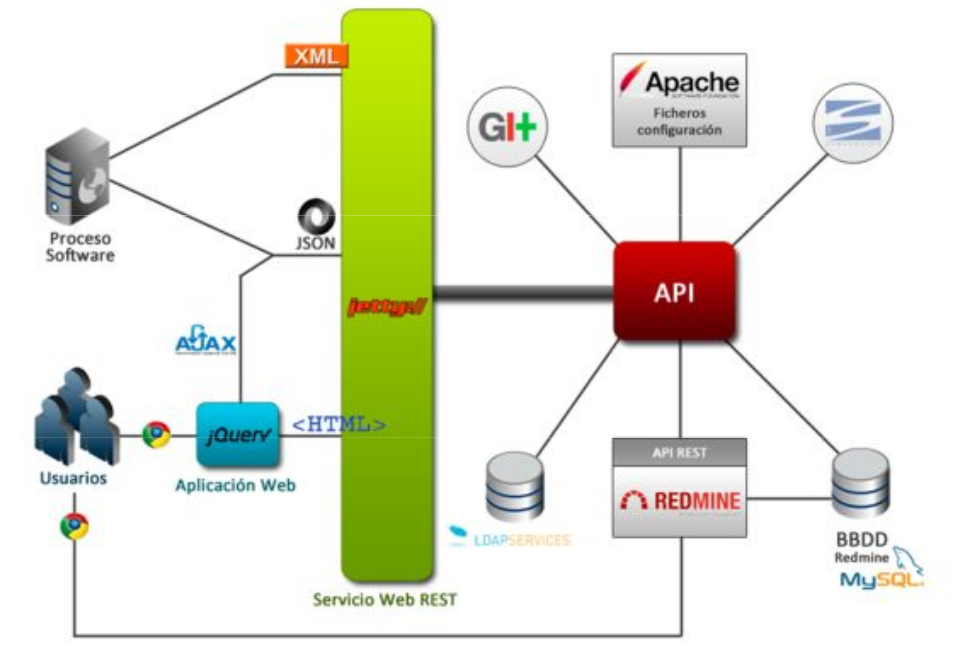
\includegraphics[width=0.7\textwidth]{arquitectura-base}
    \caption{Arquitectura SidelabCode Stack}
    \label{fig:arquitectura-scstack}
\end{figure}

%%%%%%%%%%%%%%%%%%%%%%%%%%%%%%%%%%%%%%%%%%%%%%%%%%%%%%%%%%%%%%%%%%%%%%%%%%%%%%%%%%%%%%%%%%%%%%%%%%%%%%%%%%
% OpenLDAP
%%%%%%%%%%%%%%%%%%%%%%%%%%%%%%%%%%%%%%%%%%%%%%%%%%%%%%%%%%%%%%%%%%%%%%%%%%%%%%%%%%%%%%%%%%%%%%%%%%%%%%%%%%

\subsection{Usuarios, roles y grupos}
\label{sub:usuarios-roles-grupos}

\par Gestión de usuarios, roles, grupos y proyectos a través de \emph{OpenLDAP}\footnote{OpenLDAP - \url{http://www.openldap.org/}}.

\begin{figure}[H]
    \centering
    
\includegraphics[width=0.3\textwidth]{OpenLDAP-logo}
    \caption{OpenLDAP logo}
    \label{fig:openldap-logo}
\end{figure}

\par SCStack utiliza la tecnología de directorios \emph{LDAP} como sistema de autenticación y de información centralizado de la Forja Software. En dicho servidor de directorios se almacena información relativa a todos los usuarios, proyectos software y repositorios de la Forja. Esta tecnología, además, cuenta con la ventaja de que la mayoría de aplicaciones web con sistemas de autenticación ofrecen interfaces que garantizan una completa integración con directorios LDAP, este es el caso de Redmine, Drupal, Wordpress y el propio servidor web Apache. La implementación de este protocolo en la Forja Sidelab se lleva a cabo mediante un servidor de directorios muy estable y de libre distribución que es OpenLDAP.

\subsection{API OpenLDAP}
\label{sub:api-openldap}

\par Debido a que el directorio LDAP es la estructura de información centralizada de la Forja, cualquier tipo de acción que se quiera realizar sobre el sistema requerirá el acceso por parte de la API a este servicio de directorios, bien para la recuperación de datos en las consultas o para la manipulación de registros a la hora de crear, editar o borrar usuarios o proyectos.

\par Todas las acciones de la Consola de Administración pasan a través de la API que comunica con OpenLDAP dando acceso y generando las distintas autenticaciones en cada una de las herramientas interconectadas basándose en los registros de OpenLDAP como generador y autenticador de credenciales.

% subsection api-openldap (end)

% subsection usuarios-roles-grupos (end)

%%%%%%%%%%%%%%%%%%%%%%%%%%%%%%%%%%%%%%%%%%%%%%%%%%%%%%%%%%%%%%%%%%%%%%%%%%%%%%%%%%%%%%%%%%%%%%%%%%%%%%%%%%
% Gestión de Requisitos - Redmine
%%%%%%%%%%%%%%%%%%%%%%%%%%%%%%%%%%%%%%%%%%%%%%%%%%%%%%%%%%%%%%%%%%%%%%%%%%%%%%%%%%%%%%%%%%%%%%%%%%%%%%%%%%

\subsection{Gestión de Requisitos ITS}
\label{sub:its}

\par La gestión de requisitos en SidelabCode Stack se lleva a cabo a través del Issue Tracking System \emph{Redmine}\footnote{Redmine - \url{http://www.redmine.org/}}.

\begin{figure}[H]
    \centering
    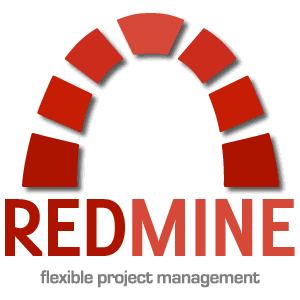
\includegraphics[width=0.3\textwidth]{redmine}
    \caption{Redmine logo}
    \label{fig:redmine-logo}
\end{figure}

\par Este apartado es el más cuidado e importante en el conjunto de SCStack ya que se trata de la herramienta encargada de centralizar la gestión de \emph{Lista de Control del Proyecto} por cada Iteración. El ITS Redmine es una aplicación web de gestión de proyectos Software multiplataforma desarrollada en \emph{Ruby} a través de \emph{Ruby on Rails}. Por supuesto se trata de una herramienta FLOSS.

\par Redmine proporciona la gestión de tareas (de cualquier tipo; \emph{features, bugs, parches\ldots}) para cada uno de los proyectos creados. Dentro de SCStack se encuentra enlazado a la configuración de usuarios a través de OpenLDAP para la validación y cuenta con una base de datos propia \emph{MySQL}. Un apartado importante ya que esto permite gestionar las migraciones de Redmine de manera rápida, eficiente y fluida de una versión a otra o incluir la información de otro Redmine\footnote{Upgrading Redmine - \url{http://www.redmine.org/projects/redmine/wiki/RedmineUpgrade}} en una nueva instalación de la Forja, únicamente haciendo un backup de la base de datos y algunos directorios clave. Incluso la migración a Redmine desde otros gestores de tareas\footnote{Migrate to Redmine - \url{http://www.redmine.org/projects/redmine/wiki/RedmineMigrate}}.

\par Proporciona una interfaz adaptada para cada proyecto de la forja asociado a un repositorio de código fuente con un visor integrado. Se visualizan los cambios entre distintas versiones del código y comparaciones entre distintas ramas de desarrollo para seguir la evolución del proyecto.

\begin{figure}[H]
    \centering
    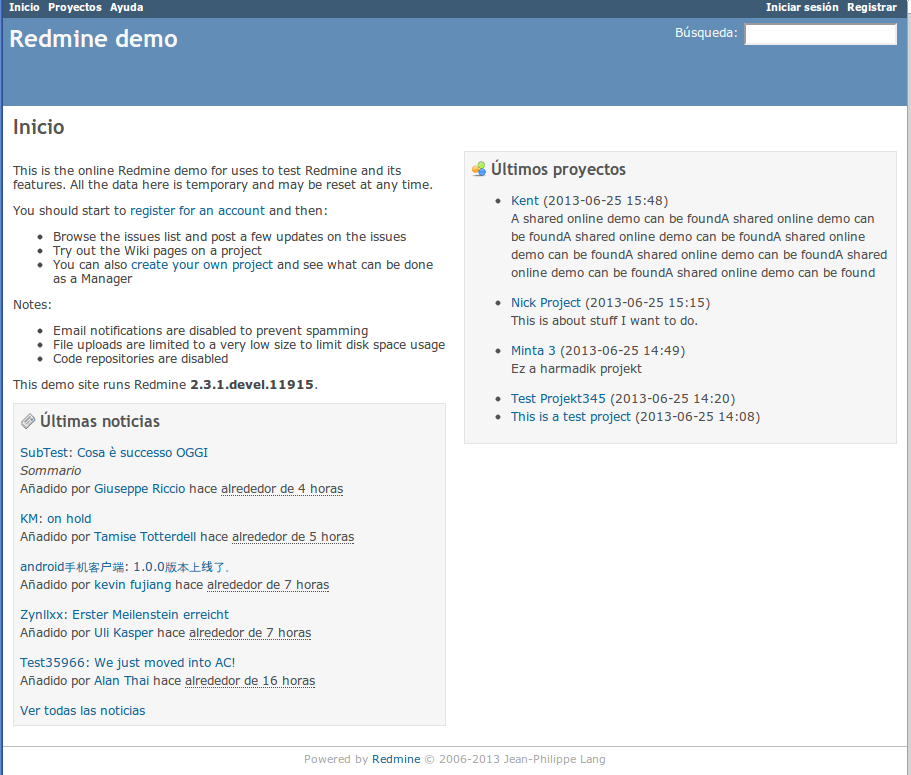
\includegraphics[width=0.7\textwidth]{redmine-demo-landing-page}
    \caption{Redmine página de bienvenida}
    \label{fig:redmine-demo-landing-page}
\end{figure}

\par Dentro del proceso Iterativo e Incremental como herramientas nos proporciona informes de seguimiento de actividad dinámicos (\emph{día, persona, proyecto\ldots}), un \emph{Wiki} para la documentación y una página de noticias.

\par Es la interfaz web de entrada al proyecto para los desarrolladores, por ello es la parte más importante y en donde se centran gran parte de los esfuerzos para la fluidez y la importancia que tiene la misma.

\par Por otra parte Redmine proporciona una API Rest para facilitar la interoperabilidad entre los distintos componentes. Esta API se maneja a través de la capa de negocio de la Consola de Administración de SCStack para así a través del API se registren en Redmine los usuarios, proyectos y grupos con sus respectivos permisos partiendo de los valores introducidos a través de la Consola de Administración. De esta forma, Redmine pasa a gestionar a través de su BBDD MySQL los usuarios y proyectos después que se hayan autenticado a través de OpenLDAP para así cargar la configuración obtenida de su BBDD.

\par Las operaciones de gestión administrativa en Redmine permanecen desactivadas, de modo que ningún administrador de proyectos puede añadir ni borrar miembros de sus proyectos, tampoco pueden crearse ni borrarse usuarios o proyectos, etc. \emph{Obligando} así que todas las operaciones de gestión de la Forja se lleven a cabo desde el Software diseñado específicamente para ello, la Consola de Administración, garantizando así la consistencia.

\subsection{Plugins}
\label{sub:redmine-plugins}

\par A la hora de aplicar el desarrollo Iterativo e Incremental se intenta incrementar la eficacia, la visibilidad, la rapidez y la comprensión del proceso de desarrollo. Por eso se han utilizado distintos plugins para Redmine que ayudan a la comprensión y agilizan el proceso Iterativo e Incremental para los usuarios (desarrolladores, gestores, etc\ldots) a través del plugin FLOSS \emph{Backlogs}\footnote{Redmine Backlogs - \url{http://www.redminebacklogs.net/}}.

\par \emph{Backlogs} aporta una gestión visual en modo tablón de las Iteraciones activas en el proceso. Gestiona 'manualmente' a través de \emph{Drag and Drop} la organización de las tareas del proyecto y agiliza la comprensión del estado de la iteración, proyecto, desarrollo en sí, en un sólo vistazo ~\ref{fig:backlogs-plugin}.

\begin{figure}[H]
    \centering
    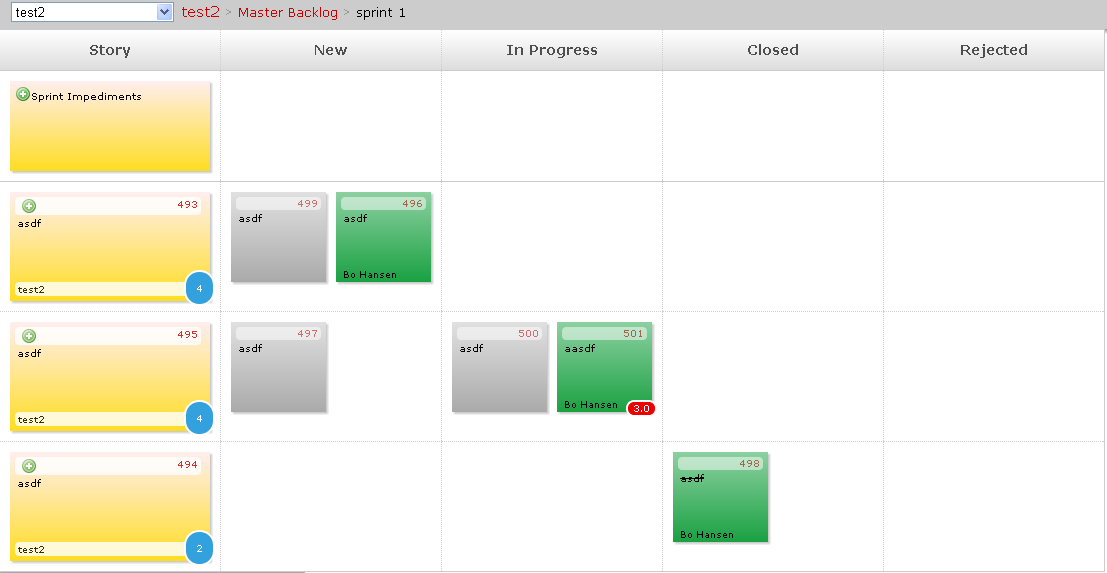
\includegraphics[width=0.7\textwidth]{backlogs-plugin}
    \caption{Redmine Backlogs plugin: tareas Redmine agrupadas por estados dentro de una historia de usuario.}
    \label{fig:backlogs-plugin}
\end{figure}

\par Otro apartado importante en el desarrollo Iterativo e Incremental es la gestión de la documentación, en este caso Redmine nos proporciona una Wiki por cada proyecto. Una Wiki es una herramienta para la documentación colaborativa que mantiene su histórico de cambios (asociados a usuario y tiempo) y que mediante el lenguaje de marcado wiki desde el cual se exportan a distintos formatos como: \emph{html, pdf, etc}, a un coste de recursos bajo ya que se trata de texto plano. El caso más famoso del uso de Wikis como documentación colaborativa es la \emph{Wikipedia}\footnote{Wikipedia - \url{http://www.wikipedia.org}}.

% subsection redmine-plugins (end)

% subsection its (end)

%%%%%%%%%%%%%%%%%%%%%%%%%%%%%%%%%%%%%%%%%%%%%%%%%%%%%%%%%%%%%%%%%%%%%%%%%%%%%%%%%%%%%%%%%%%%%%%%%%%%%%%%%%
% Repositorios de Código
%%%%%%%%%%%%%%%%%%%%%%%%%%%%%%%%%%%%%%%%%%%%%%%%%%%%%%%%%%%%%%%%%%%%%%%%%%%%%%%%%%%%%%%%%%%%%%%%%%%%%%%%%%

\subsection{Repositorios de Código}
\label{sub:repositorios}

\par Los repositorios de código (VCS) son los encargados de gestionar el ciclo de vida del código fuente como hemos visto en el apartado de Código versionado~\ref{sec:codigo-versionado} y existen dos tipos: centralizados y distribuidos. Para el proceso de desarrollo Iterativo e Incremental hemos seleccionado el repositorio distribuido \emph{Git}\footnote{Git - \url{http://git-scm.com/}}.

\begin{figure}[H]
    \centering
    
\includegraphics[width=0.3\textwidth]{git-logo}
    \caption{Git SCM Logo}
    \label{fig:git-scm-logo}
\end{figure}

\par Atendiendo a los requerimientos del proceso:

\begin{quote}
    \emph{El desarrollo de la solución se adapta al uso del Repositorio distribuido, ya que éste aporta una flexibilidad para la gestión de bifurcaciones del código que en un repositorio centralizado no tenemos fácilmente}
\end{quote}

\par En el proceso Iterativo e Incremental abundan las ramificaciones del código en el repositorio debido a ello se opta por la elección del repositorio distribuido Git en pro del repositorio centralizado SVN, que también se incluye en la Forja SCStack. Las ramificaciones, la cantidad de fusiones entre ramas~\cite{featurebranch}, entornos de desarrollo sumando la facilidad, agilidad y el bajo coste en Git nos proporcionan la herramienta adecuada para la gestión del código fuente en SCStack.

\begin{figure}[H]
    \centering
    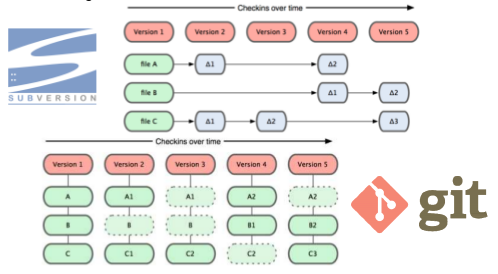
\includegraphics[width=0.7\textwidth]{svn-git-comparison}
    \caption{Comparación de incrementos entre SVN (completo) y Git (incrementos en archivos)}
    \label{fig:svn-git-comparison}
\end{figure}

\begin{quotation}
    \emph{For example the Mozilla repository is reported to be almost 12 Gb when stored in SVN using the fsfs backend. Previously, the fsfs backend also required over 240,000 files in one directory to record all 240,000 commits made over the 10 year project history. This was fixed in SVN 1.5, where every 1000 revisions are placed in a separate directory. The exact same history is stored in Git by only two files totaling just over 420 Mb. This means that SVN requires 30x the disk space to store the same history}\footnote{Git Svn Comparison Smaller Space Requirements - \url{https://git.wiki.kernel.org/index.php/GitSvnComparison\#Smaller\_Space\_Requirements}}
\end{quotation}

\par Asociada a cada Iteración se ha de gestionar la viabilidad de una rama del repositorio. En esta rama se trabaja con respecto a las tareas a desarrollar para la iteración. Se hacen las pruebas necesarias para cada desarrollo para después integrar la solución en la rama principal y así crear una nueva versión del proyecto. 

\par La ramificación del desarrollo permite gestionar por iteraciones incrementales aisladas en una nueva rama, de esta forma, el contenido de la rama principal es fiable, ya que para añadir contenido a la rama ha tenido que pasar una iteración nueva y el proceso de desarrollo que conlleva; planificación, test, implementación e integración. El resultado está altamente controlado y distribuido en base a módulos para poder acotar posibles errores posteriores o revertir cambios a través de un proceso minuciosamente controlado.

% subsection repositorios (end)

\subsection{Revisión de Código}
\label{sub:gerrit}

\par Gerrit.

% subsection gerrit (end)

%%%%%%%%%%%%%%%%%%%%%%%%%%%%%%%%%%%%%%%%%%%%%%%%%%%%%%%%%%%%%%%%%%%%%%%%%%%%%%%%%%%%%%%%%%%%%%%%%%%%%%%%%%
% Integración Continua
%%%%%%%%%%%%%%%%%%%%%%%%%%%%%%%%%%%%%%%%%%%%%%%%%%%%%%%%%%%%%%%%%%%%%%%%%%%%%%%%%%%%%%%%%%%%%%%%%%%%%%%%%%

\subsection{Integración Continua}
\label{sub:ci-jenkins}

\par Jenkins CI.

% subsection ci-jenkins (end)

\subsection{Gestión de distribuciones y dependencias.}
\label{sub:distribuciones-dependencias}

\par Directorios compartidos, OpenSSH y Archiva para la gestión de dependencias.

% subsection distribuciones-dependencias (end)

% subsection componentes (end)

%%%%%%%%%%%%%%%%%%%%%%%%%%%%%%%%%%%%%%%%%%%%%%%%%%%%%%%%%%%%%%%%%%%%%%%%%%%%%%%%%%%%%%%%%%%%%%%%%%%%%%%%%%
% Desarrollo Eclipse y Maven
%%%%%%%%%%%%%%%%%%%%%%%%%%%%%%%%%%%%%%%%%%%%%%%%%%%%%%%%%%%%%%%%%%%%%%%%%%%%%%%%%%%%%%%%%%%%%%%%%%%%%%%%%%

\subsection{Desarrollador: Eclipse y Maven}
\label{sub:eclipse-mvn-tdd}

\par El entorno de desarrollo para el desarrollador en el que se integra el proceso Iterativo e Incremental consta de dos herramientas y un concepto.

\par El IDE \emph{Integrated Development Environment} a utilizar es Eclipse, concretamente la distribución del framework Spring \emph{Eclipse STS}\footnote{Eclipse STS - \url{http://www.springsource.org/sts}}. 

\begin{figure}[H]
    \centering
    
\includegraphics[width=0.3\textwidth]{STS}
    \caption{Spring Tool Suite logo}
    \label{fig:sts}
\end{figure}

\par STS otorga y proporciona un conjunto de herramientas preparadas para trabajar con los componentes de STStack: Redmine, Git, Gerrit, Jenkins, Apache, OpenLDAP, Maven. Se basa en unan distribución de Eclipse orientada al desarrollo para trabajar con diferentes componentes externos facilitando la puesta a punto para empezar a desarrollar.

\par Esta distribución incluye la gestión de un proyecto a través \emph{Maven}\footnote{Apache Maven - \url{http://maven.apache.org/}}. Maven es un Software de gestión de proyectos basado en la definición del proyecto POM (Project Object Model). Es el encargado de compilar, ejecutar test, desplegar, gestionar las dependencias (locales y remotas) y generar distribuciones a partir de una configuración definida.

\begin{figure}[H]
    \centering
    
\includegraphics[width=0.3\textwidth]{maven}
    \caption{Maven logo}
    \label{fig:maven-logo}
\end{figure}

\par Esta herramienta se integra en el ciclo de vida del Software para automatizar los procesos tediosos manuales, proveer una estructura básica inicial a los proyectos (iteración 0) para ir incrementando iteración tras iteración a través de los arquetipos.

\par A través de Maven y Eclipse se definen las líneas del desarrollo de cada iteración facilitando el diseño TDD~\ref{sub:tdd} a través de una sencilla configuración. El esqueleto de los proyectos Maven proporciona unas sencillas guías estándar para el desarrollo de proyectos de Software. Esta agrupación de funcionalidades se reutiliza en Jenkins-CI a través de los jobs de Maven para así poder replicar cualquier entorno durante la integración continua partiendo de una base robusta.

% subsection mv-tdd (end)

%%%%%%%%%%%%%%%%%%%%%%%%%%%%%%%%%%%%%%%%%%%%%%%%%%%%%%%%%%%%%%%%%%%%%%%%%%%%%%%%%%%%%%%%%%%%%%%%%%%%%%%%%%
% Interoperabilidad
%%%%%%%%%%%%%%%%%%%%%%%%%%%%%%%%%%%%%%%%%%%%%%%%%%%%%%%%%%%%%%%%%%%%%%%%%%%%%%%%%%%%%%%%%%%%%%%%%%%%%%%%%%

\section{Interoperabilidad}
\label{sec:interoperabilidad}

\par Interoperabilidad entre las herramientas que componen la forja. API Rest.

% section interoperabilidad (end)

%%%%%%%%%%%%%%%%%%%%%%%%%%%%%%%%%%%%%%%%%%%%%%%%%%%%%%%%%%%%%%%%%%%%%%%%%%%%%%%%%%%%%%%%%%%%%%%%%%%%%%%%%%
% Pruebas y Validación
%%%%%%%%%%%%%%%%%%%%%%%%%%%%%%%%%%%%%%%%%%%%%%%%%%%%%%%%%%%%%%%%%%%%%%%%%%%%%%%%%%%%%%%%%%%%%%%%%%%%%%%%%%

\section{Pruebas y Validación}
\label{sec:pruebas-validacion}

\par Pruebas a trav\'es de virtualizaci\'on de sistemas operativos mediante herramientas libres; Vagrant, kvm, puppet.

% section pruebas-validacion (end)
